\chapter{Applicazione lineari e prodotto di matrici}
\section{Applicazioni lineari: definizione e esempi\label{applin}}
Inizieremo ora a parlare di funzioni tra spazi vettoriali. Ricordiamo che una funzione $f:X\to Y$ tra due insiemi
$X$ (detto \textit{dominio}) e $Y$ (detto \textit{codominio}) è una legge che associa a ogni $x\in X$ un ben
preciso elemento di $Y$, detto \textit{immagine di $x$} e denotato $f(x)$.\\
Noi studiaeremo le funzioni $f:V\to W$ in cui dominio e codominio $V$ e $W$ sono spazi vettoriali su un certo
campo $\mathds{K}$, e in particolare studieremo quelle che soddisfano la seguente
\begin{definizione}
  Una funzione $f:V\to W$ tra spazi vettoriali si dice \texttt{funzione lineare} (o \textit{applicazione
    lineare}) se verifica le due seguenti proprietà:
  \begin{eqnarray}
    \label{4.1-4.2}
    f(v+v^{\prime})=f(v)=f(v^\prime) \text{ per ogni } v,v^\prime \in V\\
    f(cv)=cf(v) \text{ per ogni } v\in V\text{ e ogni scalare }c \in \mathds{K}
  \end{eqnarray}
  Limitarsi alla funzione lineare può sembrare molto restritivo:
  \begin{esempio}
    si può vedere che se\footnote{Sappiamo che $\mathds{R}^n$ è una spazio vettoriale di dimensione $n$, in
      particolare per $n=1$ si ottiene $\mathds{R}^1=\mathds{R}$ (che risulta quindi spazio vettoriale come da
      dimostrazione 1).}  $V=W=\mathds{R}$, le uniche funzioni lineari $f:\mathds{R}\to\mathds{R}$ sono quelle
    del tipo $f(x)=ax$, con $a\in \mathds{R}$ fissato.
  \end{esempio}
  Tuttavia, vediamo subito che tra le applicazioni lineari vi sono funzioni di grante impotanza e utilità in
  geometria e nello sue applicazioni:
  \begin{esempio}
    Dato lo spazio $V_O^2$ dei vettori geometrici applicati nel piano, consideriamo la funzione
    $f:V_O^2\to V_O^2$ che associa a ogni vettore $\vec{OP}$ il vettore che si ottiene ruotando $\vec{OP}$ di
    un angolo $\theta$ fissato in senso antiorario attorno all'origine $O$,come nel disegno sequente 
    \begin{figure}[th]
      \centering
        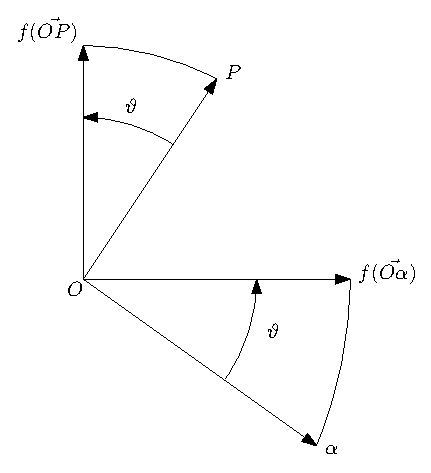
\includegraphics[width=5cm]{img/finiti/imgex4-2-1.eps}
      \caption{$f:V_O^2\to V_O^2$}
    \end{figure}
    Ora, come si vede nel disegno sequente, dati due vettori $\vec{OP}$ e $\vec{OP}^\prime$, sommarli e poi
    ruotare il vettore risultante oppure prima ruotarli e poi sommare i vettori ruotati è equivalente, ovvero
    \clearpage
    \begin{figure}[th]
      \centering
        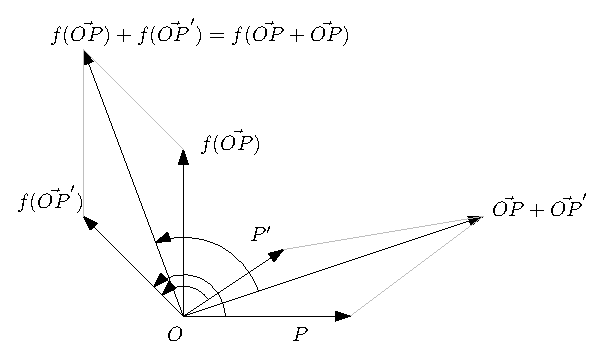
\includegraphics[width=6cm]{img/finiti/imgex4-2-2.eps}
      \caption{$f(\vec{OP})+f(\vec{OP}^\prime)=f(\vec{OP}+\vec{OP})$}
    \end{figure}
    Quindi vale la
    \begin{equation}
      f(\vec{OP})+f(\vec{OP}^\prime)=f(\vec{OP}+\vec{OP})
    \end{equation}
    che ci dice che questa funzione soddisfala proprietà (\ref{applin}) della Definizione \ref{4.1-4.2}\\
    Analogamente, dato un vettore $\vec{OP}$ e un numero reale $c$, moltiplicare il vettore per $c$ e poi
    ruotarlo e poi moltiplicarlo per $c$ è equivalente:
    \begin{figure}[th]
      \centering
        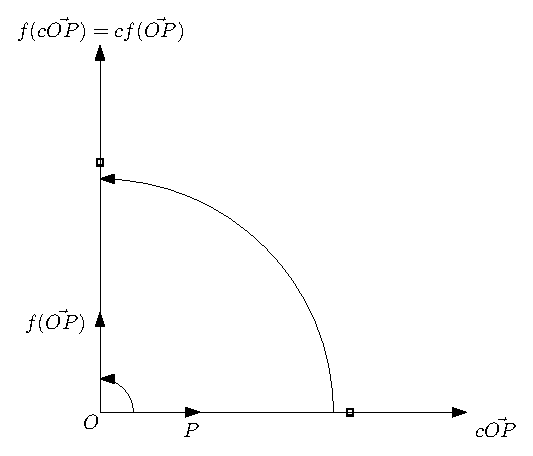
\includegraphics[width=6cm]{img/finiti/imgex4-2-3.eps}
      \caption{$f(c\vec{OP})=cf(\vec{OP})$}
    \end{figure}
    Quindi si ha
    \begin{equation}
      f(c\vec{OP})=cf(\vec{OP})
    \end{equation}
    che ci dice che questa funzione soddisfa anche la proprietà (\ref{matasapplin}), della definizione
    \ref{4.1-4.2} -- Concludiamo quindi che le rotazioni attorno a $O$ sono applicazioni lineari dallo
    spazio vettoriale $V_O^2$ in se stessso.\\
    Possiamo arrivare alla stessa conclusione anche per altre importanti trasformazioni geometriche: ad
    esempio, si consideri la riflessione rispetto a una retta $r$ passante per $O$, che manda ogni vettore
    $\vec{OP}\in V_O^2$ nel vettore simmetrico rispetto alla retta, come nel seguente disegno
    \begin{figure}[th]
      \centering
        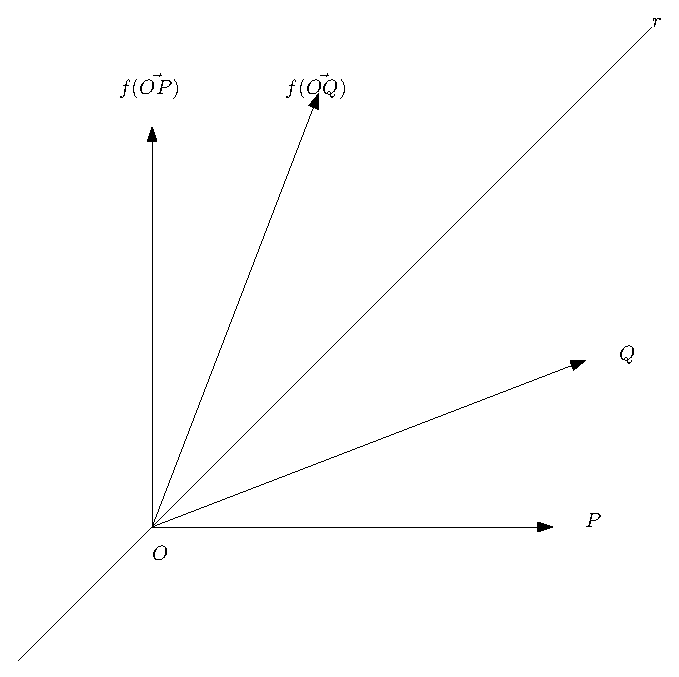
\includegraphics[width=6cm]{img/finiti/imgex4-2-4.eps}
    \end{figure}   
    Allora, come già fatto per le rotazioni, notiamo che, dati due vettori $\vec{OP}$ e $\vec{OP}^\prime$,
    sommarli e poi riflettere il vettore risultante oppure prima rifletterli e poi sommare i vettori riflessi
    è equivalente
    \clearpage
    \begin{figure}[th]
      \centering
        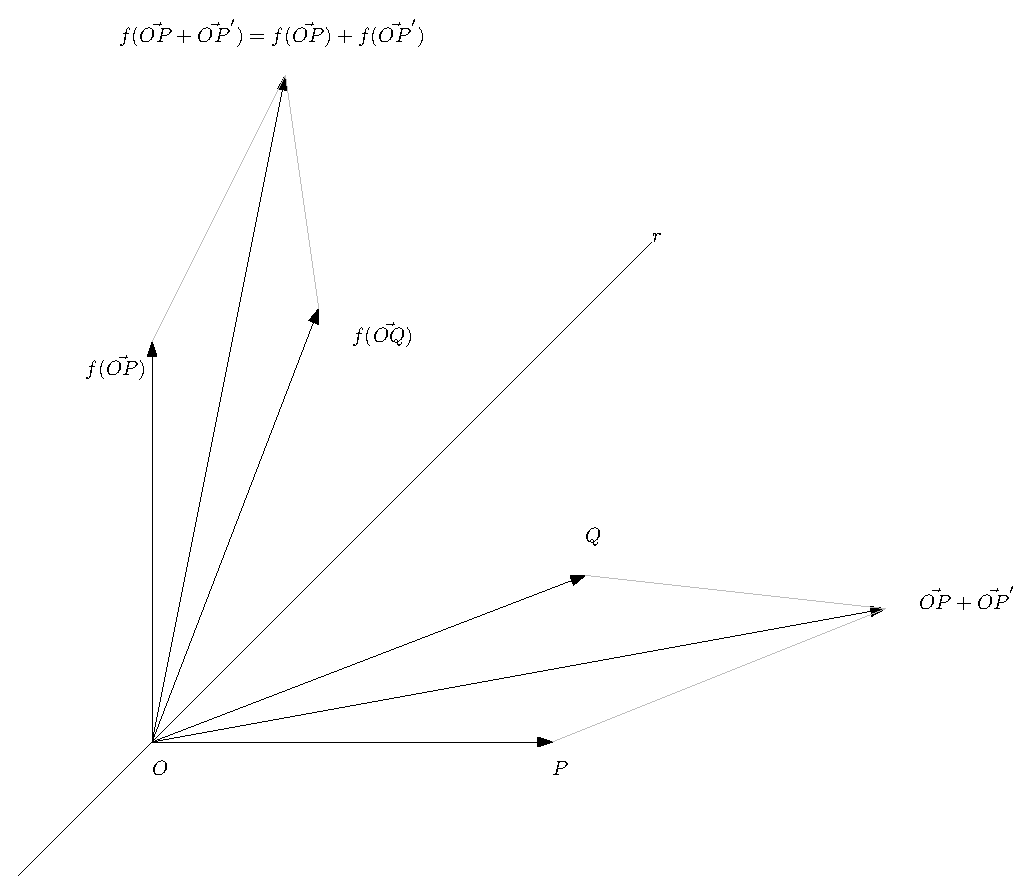
\includegraphics[width=6cm]{img/finiti/imgex4-2-5.eps}
    \end{figure}
    $f\left(\vec{OP}+\vec{OP}^\prime\right)=f\left(\vec{OP}\right)+f\left(\vec{OP}^\prime\right)$ e
    dato uin vettore $\vec{OP}$ e un numero
    reale $c$, moltiplicatore il vettore per $c$ e poi rifletterlo oppure prima rifletterlo e poi moltiplicarlo
    per $c$ è equivalente
    \begin{figure}[th]
      \centering
        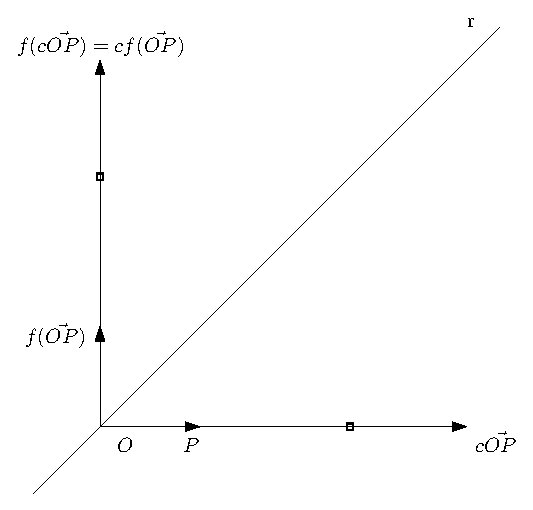
\includegraphics[width=6cm]{img/finiti/imgex4-2-6.eps}
    \end{figure}
      
    $f(c\vec{OP})=cf(\vec{OP})$: quindi concludiamo che anche la riflessione rispetto a una retta ce passa per
    $O$, avendo le proprietà entrambe le proprietà (\ref{4.1-4.2}) richieste nella Definizione (\ref{applin}),
    è un'applicazione lineare $f:V_O^2\to        V_O^2$.\\
    Come terzo esempio esempio di applicazione lineare $V_O^2\to V_O^2$ citiamo la propiezione ortogonale,
    che proieta ortogonalmente i vettori su una retta fissata passante per $O$.
    \begin{figure}[th]
      \centering
        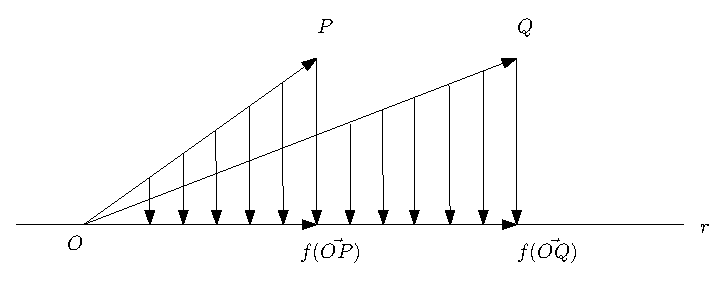
\includegraphics[width=8cm]{img/finiti/imgex4-2-7.eps}
    \end{figure}
      
    per la quale è difficile vedere che valgono ancora le proprieta citate in (\ref{4.1-4.2}).\\
    Analogamente a quanto visto per rotazioni, riflessioni e proiezioni nel piano, anche le corrispondenti
    trasformazioni $V_O^3\to V_O^3$ dello spazio tridimensionale come da proprietà (\ref{4.1-4.2}) della
    Definizione \ref{applin} la rotazione di un angolo fissato $\Theta$ attorno a una retta data passante per $O$
    (detta ase della rotazione)
    \clearpage
    \begin{figure}[th]
      \centering
        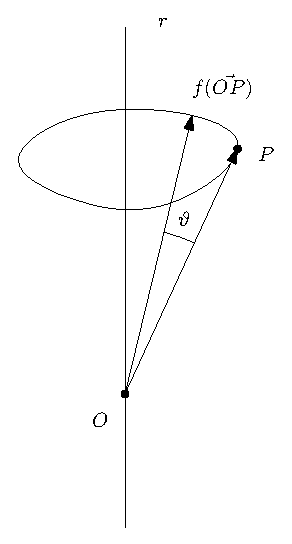
\includegraphics[width=3cm]{img/finiti/imgex4-2-8.eps}
    \end{figure}
    la riflessione rispetto a un piano passante per $O$
    \begin{figure}[th]
      \centering
        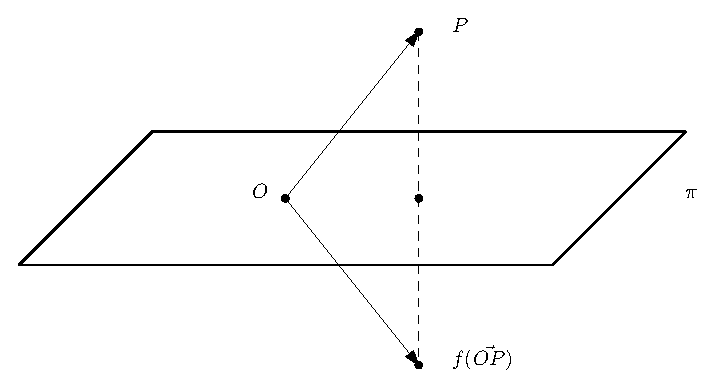
\includegraphics[width=6cm]{img/finiti/imgex4-2-9.eps}
    \end{figure}
      
    e la proiezione ortogonale su un piano passante per l'origine $O$:
    \begin{figure}[th]
      \centering
        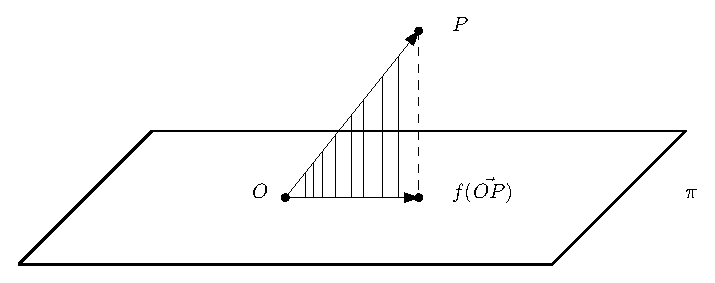
\includegraphics[width=6cm]{img/finiti/imgex4-2-10.eps}
    \end{figure}
    (Quest'ultima può anche essere vista come applicazione $f:V_O^3\to V_O^2$ se vediamo il piano su cui
    proiettiamo come spazio vettoriale a se stante).
  \end{esempio}
\end{definizione}

\section{Matrice associata a un'applicazione lineare}
Una delle caratteristiche fondamentali di un'applicazione lineare $f:V\to W$ è che, se gli spazi $V$ e $W$ hanno
dimensione finita, allora $f$ può essere rappresentata da una matrice.\\ Vediamo i dettagli: sia $f:V\to W$
un'applicazione lineare, e siamo $B_V=\left\{v_1,v_2,\dots,v_n\right\}$ e $B_W=\left\{w_1,w_2,\dots,w_n\right\}$
basi di $V$ e $W$ rispettivamente. Allora, come sappiamo ogni vettore $v\in V$ può essere identificato con una
$n-$upla $\left(x_1,x_2,\dots,x_n\right)$, quella delle sua coordinate rispetto alla base $B_V$ (ovvero
$v=x_1v_1+x_2v_2+\dots+x_nv_n$), e analogamente ogni vettore $w\in W$ può rispetto alla base $B_W$ (ovvero
$w=y_1w_1+y_2w_2+\dots+y_mw_m$). Con questo identificazioni, la $f$ può essere pensata come una funzione
$\mathds{K}^n\to\mathds{K}^m$ che associa a ogni $n$-upla. Ci proponiamo di trovare l'espressione esplicita di
tale funzione. A questo scopo, sia $(x_1,\dots,x_n)$ la $n$-upla delle coordinate di un vettore $v\in V$, ovvero
come abbiamo ricevuto sopra $v=x_1v_1+\dots+x_nv_n$. Allora la sua immagine $f(v)$ sarà
\begin{equation*}
  f(v)=f(x_1v_1+\dots+x_nv_n) =
\end{equation*}
(usando le proprietà un'applicazione lineare)
\begin{equation}
  =f(x_1v_1)+\dots+f(x_nv_n)=x_1f(v_1)+\dots+x_nf(v_n).
\end{equation}
Ora, ciascuno dei vettori $f(v_1),f(v_2),\dots,f(v_n)$ che compare nella ({\bf 4.5}) appartiene al codominio $W$
della funzione, e quindi potrà essere espresso come combinazione lineare dei vettori $w_1,w_2,\dots,w_m$ della
base $B_W$ fissata per $W$:
\clearpage
\begin{equation}
  f(v_1)=a_{11} w_1+a_{21}w_2+\dots+a_{m1}w_m
\end{equation}
\begin{equation*}
  \vdots
\end{equation*}
\begin{equation}
  f(v_1)=a_{1n} w_1+a_{2n}w_2+\dots+a_{mn}w_m
\end{equation}
Ora, sostituendo queste espressioni nella ({\bf 4.5}) si ottiene
\begin{equation*}
  f(v)=x_1(a_{11} w_1+a_{21}w_2+\dots+a_{m1}w_m) +\dots+ x_n(a_{1n} w_1+a_{2n}w_2+\dots+a_{mn}w_m)=
\end{equation*}
(svolgendo i conti e mettendo in evidenza i vettori)
\begin{equation}
  =(a_{11}x_1+\dots+a_{1n}x_n)w_1+\dots+(a_{m1}x_1+\dots+a_{mn}x_n)w_m
\end{equation}
Questa uguaglianza ci sta dicendo che le coordinate del vettore $f(v)$ rispetto alla base $B_W=\left\{w_1,w_2,
  \dots,w_m\right\}$ sono date da $a_{11}x_1+\dots+a_{1n}x_n,\dots,a_{m1}x_1+\dots+a_{mn} x_n$ e quindi che,
tradotta in coordinate, la nostra applicazione lineare può essere identificata con la funzione $\mathds{K}^n\to
\mathds{K}^m$ che associa a ogni $n$-upla $(x_1,\dots,x_n)$ la $m$-upla formata dai coefficienti che appiono nella
({\bf 4.8}), ovvero
\begin{equation}
  \begin{pmatrix}
    x_1\\
    x_2\\
    \vdots\\
    x_n
  \end{pmatrix} \to
  \begin{pmatrix}
    a_{11}x_1+a_{12}x_2+\dots+a_{1n}x_n\\
    a_{21}x_1+a_{22}x_2+\dots+a_{2n}x_n\\
    \vdots\\
    a_{m1}x_1+a_{m2}x_2+\dots+a_{mn}x_n
  \end{pmatrix}
\end{equation}
I coefficienti che compaiono nella ({\bf 4.9}) formano una matrice con $m$ righe e $n$ colonne
\begin{equation*}
  A=
  \begin{pmatrix}
    a_{11} &a_{12}&\dots&a_{1n}\\
    a_{21} & a_{22}&\dots& a_{2n}\\
    \dots\\
    a_{m1} & a_{m2} &\dots&a_{mn}
  \end{pmatrix}
\end{equation*}
che chiamaremo la \textit{matrice associata all'applicazione lineare rispetto alle basi $B_V$ e $B_W$}. In base
alle (\textbf{4.6}), \dots{}, (\textbf{4.7}) tale matrice può essere definita come \textit{la matrice che ha sulle
  colonne le coordinate dei vettori $f(v_1),\dots,f(v_n)$ (ovvero le immagini dei vettori della base $B_V$
  fissata nel dominio) rispetto alla base $B_W$ fissata nel codominio}.\\
Denoteremo $M_{B_wB_V}(f)$ la matrice associata a un'applicazione lineare $f:V\to W$ rispetto alle basi $B_V$ e
$B_W$.\\
Se dominio e codomio dell'applicazione coincidono, ovvero si ha una funzione linerare $f:V\to V$ (tale
applicazione si dicono \textit{endomorfismi}), allora è possibile fissare la stessa base $B_V$ sia nel dominio
che nel codominio, e calcolare la matrice associata $M_{B_wB_V}(f)$. Come vedremo, la matrice associata a
un'applicazione lineare ci dà tutte le informazioni di cui abbiamo bisogno sull'applicazione, e usando gli
strumenti imparati nei capitoli precedenti (\textit{rango, determinante}) saremo in grado di capire molte
proprietà della funzione data. Prima di fare ciò, vediamo subito alcuni esempi di calcolo della matrice
associata.
\begin{esempio}
  \begin{enumerate}
  \item Sia $f:V_O^2\to V_O^2$ la rotazione attorno a $O$ di un angolo fissato $\Theta$\footnote{abbiamo visto nel
      nel paragrafo precedente si tratta di un'applicazione lineare}. Per calcolare la matrice associata, fissiamo
    una base $B$ formata da due vettori $=v_1=\vec{OP}_1$ e $v_2=\vec{OP}_2$ dlla stessa lunghezza e
    perpendicolari tra loro, come nel disegno
    \begin{figure}[th]
      \centering
        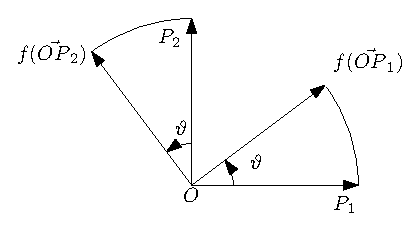
\includegraphics[width=6cm]{img/finiti/imgex4-3-1.eps}
    \end{figure}

    e determiniamo la matrice $M_B(f)$.\\
    A questo scopo, come afferma la difinizione di matrice associata dobbiamo trovare le coordinate di $f(v_1)$ e
    $f(v_2)$ rispetto a $B$, ovvero esprimere $f(\vec{OP}_1)$ e $f(\vec{OP}_2)$ come combinazione lineare
    $x_1\vec{OP}_1+x_2\vec{OP}_2$ dei vetori della base $B$. Iniziamo con $f(\vec{OP}_1)$: come si vede nel
    disegno seguente
    \clearpage
    \begin{figure}[th]
      \centering
        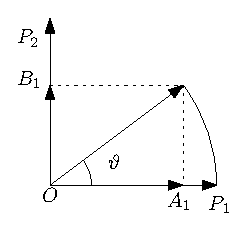
\includegraphics[width=6cm]{img/finiti/imgex4-3-2.eps}
    \end{figure}

    (nel quale stiamo denotando $R_1$ il punto finale del vettore ruotato $f(\vec{OP}_1)$) si ottine
    $f(\vec{OP}_1)=\vec{OP}_1=\vec{OA}_1+\vec{OB}_1$, essendo $A_1$ e $B_1$ le proiezioni ortogonali di $R_1$
    sui vettori di base. Ora, chiaramente $\vec{OA}_1=x_1\vec{OP}_1$ e $\vec{OB}_1=x_2\vec{OP}_2$, dove $x_1$ è
    dato dal rapporto $\frac{\abs{\vec{OA}_1}}{\vec{OP}_1}$ tra la lunghezza di $\vec{OA}_1$ e quella di
    $\vec{OP}_1$, mentre $x_2$ è dato dal rapporto $\frac{\abs{\vec{OB}_1}}{\vec{OP}_2}$ tra la lunghezza di
    $\vec{OB}_1$ e quella di $\vec{OP}_2$. Ma essendo la lunghezza di $\vec{OP}_1$ uguale alla lunghezza di
    $\vec{OR}_1=f(\vec{OP}_1)$\footnote{La rotazione non modifca la lunghezza dei vettore, essi restano
      inveriati anche se cambiano la loro angolazione.} possimo dire che $x_1$ è uguale al rapporto tra la
    lunghezza del cateto $\vec{OA}_1$ e quella dell'ipotenusa $\vec{OP}_1$ del triangolo rettangolo $OR_1A_1$,
    ovvero (esendo il cateto in questione adiacente all'angolo), $x_1=\cos\Theta$. \\
    Analogamente, poiché $\vec{OP}_1$ ha la stessa lunghezza di $\vec{OP}_1$ e quindi di $\vec{OR}_1$, mentre
    $\vec{OB}_1$ ha la stessa lunghezza del segmento $A_1R_1$, si ha 
    \begin{equation*}
      x_2=\frac{\abs{\vec{OB}_1}}{\abs{\vec{OP}_2}}=\frac{\abs{A_1R_1}}{OR_1}
    \end{equation*}
    ovvere\footnote{Essendo il rapporto tra il cateto $A_1R_1$, opposto all'angolo $\Theta$, e l'ipotenusa
      $OR_1$ del triangolo rettangolo $OR_1A_1$}, $x_2=\sin \Theta$. Riassumendo,
    \begin{equation}
      f(\vec{OP}_1)=\vec{OR}_1=\vec{OA}_1+\vec{OB}_1=\cos\Theta \vec{OP}_1+\sin \Theta \vec{OP}_2
    \end{equation}
    Ora, facciamo un ragionamento analogo per determinare $f(\vec{OP}_2)$: come si vede nel disegno seguente
    \begin{figure}[th]
      \centering
        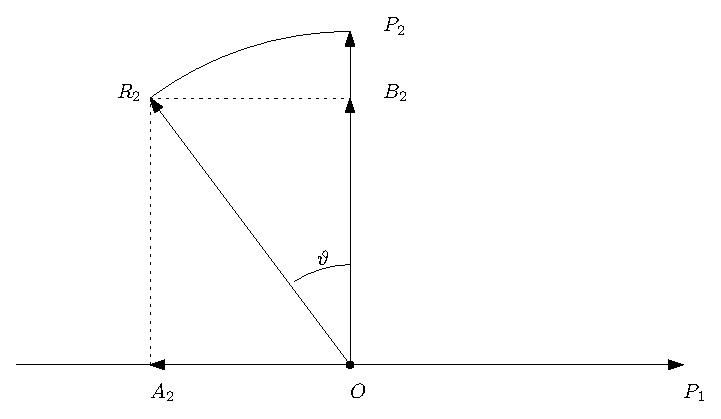
\includegraphics[width=6cm]{img/finiti/imgex4-3-3.eps}
    \end{figure}
      
    (nel quale stiamo denotando $R_2$ il punto finale del vettore ruotato $f(\vec{OPT})$) si ha
    $f(\vec{OP}_2)=\vec{OR}_2=\vec{OA_2}+\vec{OB_2}$. Ora, chiaramente $\vec{OA}_2=-x_1\vec{OP}_1$, dove $x_1$ è
    dato dal rapporto $\frac{\abs{\vec{OA}_2}}{\abs{\vec{OP}_1}}$ tra la lunghezza di $\vec{OA}_2$ e quella di
    $\vec{OP_1}$ (il segno meno è dovuto dal fatto che $\vec{OA}_2$ ha verso opposto rispetto a $\vec{OP}_1$) e
    $\vec{OB}_2=x_2\vec{OP}_2$, dove $x_2$ è dato dal rapporto $\frac{\abs{\vec{OB}_2}}{\abs{\vec{OP}_2}}$ tra la
    lunghezza di $\vec{OB}_2$ e quella di $\vec{OR}_2$. Ma essendo la lunghezza di $\vec{OP}_1$ uguale alla
    lunghezza di $\vec{OP}_1$ uguale alla lunghezza di $\vec{OP}_2$ e quindi di $\vec{OR}_2=f(\vec{OP}_2)$
    (sempre perché la rotazione non modifica la lunghezza dei vettori), mentre, la lunghezza di $\vec{OA}_2$ è
    uguale alla lunghezza del segmento $R_2B_2$, possiamo dire che $x_1$ è uguale al rapporto tra la lunghezza
    del cateto $R_2B_2$ e quella dell'ipotenusa $OR_2$ del triangolo rettangolo $OR_2B_2$, ovvero (essendo il
    cateto in questione opposto all'angolo), $x_2=\cos\Theta$.\\
    Riassumendo,
    \begin{equation}
      f(\vec{OP}_2)=\vec{OR}_2=\vec{OA}_2+\vec{OB_2}=-\sin\Theta\vec{OP}_1+\cos \Theta\vec{OP}_2
    \end{equation}
    \clearpage
    Quindi, (\textbf{4.10}) e (\textbf{4.11}) ci dicono che la matrice associata a $f$ rispetto a $B$ avrà sulla
    prima colonna $(\cos\Theta,\sin\Theta)$\footnote{le coordinate di $f(\vec{OP}_1)$ rispetto a $B$} e sulla
    seconda colonna $(-\sin\Theta,\cos\Theta)$ (le coordinate di $f(\vec{OP})$ rispetto a $B$), ovvero
    \begin{equation}
      M_B(f)=
      \begin{pmatrix}
        \cos\Theta & -\sin \Theta\\
        \sin\Theta & \cos \Theta
      \end{pmatrix}
    \end{equation}
    Come visto nel (\textbf{4.9}), abbiamo allora che la rotazione, in coordinate, si traduce nella funzione
    $f:\mathds{R}^2\to\mathds{R}^2$ data da
    \begin{equation}
      (x_1,x_2)\mapsto (\cos\Theta x_1-\sin\Theta x_2,\sin\Theta x_1+\cos\Theta x_2)
    \end{equation}
    Ad esempio, scegliamo $\Theta=\frac{\pi}{4}$ e sostituiamo in $(4.12)$ e $(4.13)$, ottenendo rispettivamente
    (si ricordi che $\cos\frac{\pi}{4}=\sin\frac{\pi}{4}=\frac{\sqrt{2}}{2}$)
    \begin{equation*}
      M_B(f)=
      \begin{pmatrix}
        \frac{\sqrt{2}}{2} & -\frac{\sqrt{2}}{2} \\
        \frac{\sqrt{2}}{2} & \frac{\sqrt{2}}{2}
      \end{pmatrix}.
    \end{equation*}
    e anche
    \begin{equation}
      (x_1,x_2)\mapsto
      \begin{pmatrix}
        \frac{\sqrt{2}}{2}x_1+\frac{\sqrt{2}}{2}x_2,\frac{\sqrt{2}}{2}x_1+\frac{\sqrt{2}}{2}x_2
      \end{pmatrix}
    \end{equation}
    Per illustrare come questa semplice funzione $\mathds{R}^2\to\mathds{R}^2$ rappresenti effettivamente la
    rotazione di $\frac{\pi}{4}$, prendiamo ad esempio il vettore $v=v_1+v_2$, che come si vede nel disegno
    seguente coincide con la diagonale del quadrato che ha $v_1$ e $v_2$ come lati:
    \begin{figure}[th]
      \centering
        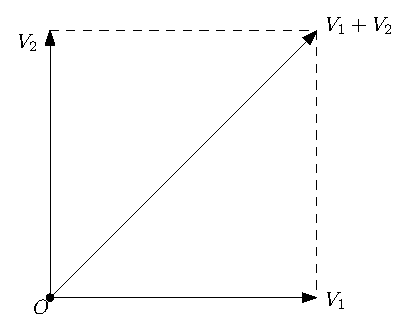
\includegraphics[width=4cm]{img/finiti/imgex4-3-4.eps}
    \end{figure}

    Tale vettore ha quindi come coordinate rispetto a $B$ la coppia $(x_1,x_2)=(1,1)$. In base alla
    \textbf{(4.14)}, le coordinate di $f(v)$ rispetto a $B$ sono date da
    \begin{equation*}
      \frac{\pi}{4}*1-\frac{\pi}{4}*1,\frac{\pi}{4}*1+\frac{\pi}{4}*1=(0,\sqrt{2})
    \end{equation*}
    ovvero deve essere $f(v)=0v_1+\sqrt{2}v_2=\sqrt{2}v_2$.\\
    In effetti, tale risultato ottenuto analicamente in coordinate è confermato dall'analisi grafica, che ci
    dice che il vettore $f(v)$ che si ottiene ruotando la diagonale $v$ del quadrato di $\frac{\pi}{4}$ è proprio
    proporzionale al vettore $v_2$ e la sua lunghezza è proprio $\sqrt{2}$ volte la lunghezza di $v_2$ (in
    quasto $v$ coincideva con la diagonale del quadrato di lati $v_1$ e $v_2$):
    \begin{figure}[th]
      \centering
        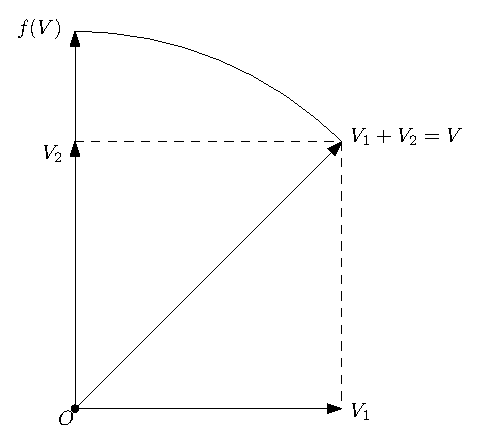
\includegraphics[width=4cm]{img/finiti/imgex4-3-5.eps}
    \end{figure}
  \item Sia $V=V_O^2$ lo spazio vettoriale dei vettori applicati in un punto $O$ nel piano e sia $f:V_o^2\to
    V_O^2$ la proiezione ortogonale su una retta fizzata $r$ passante per $O$\footnote{abbiamo visto nel
      paragrafo precedente che si tratta di un'applicazione lineare}.\\
    Ora, notiamo che quando proiettiamo $v_1$ ortogonalmente su $r$, otteniamo un vettore $v$ che sta sulla retta
    ed è lungo come metà della diagonale del quadrato i cui lati sono $v_1$ e $v_2$: essendo tale diagonale,
    per definizione di somma tra vettori, coincidente con $v_1+v_2$, abbiamo quindi che $f(v_1)=
    \frac{1}{2}(v_1+v_2)=\frac{1}{2}v_1+\frac{1}{2}v_2$; analogamente, come si vede dal disegno, anche
    proiettando $v_2$ sulla retta di ottiene lo stesso vettore $v$, quindi si ha anche $f(v_2)=
    \frac{1}{2}(v_1+v_2)=\frac{1}{2}v_1+\frac{1}{2}v_2$.
    \begin{figure}[th]
      \centering
        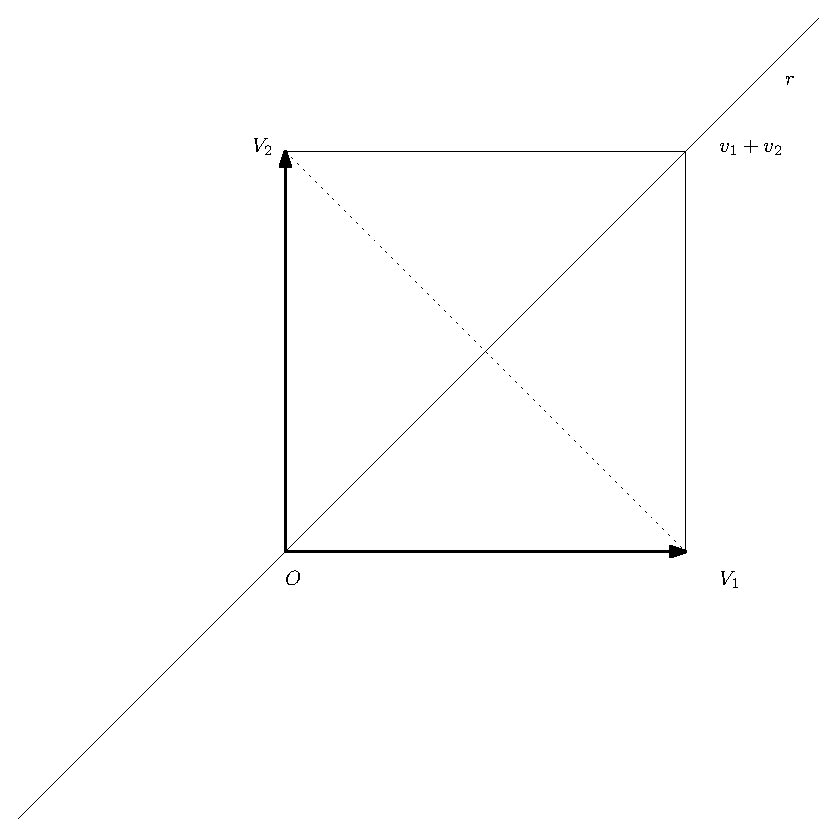
\includegraphics[width=4cm]{img/finiti/imgex4-3-6.eps}
    \end{figure}
    Si vede quindi che le coordinate di $f(v_1)$ rispetto a $B$ sono $\left(\frac{1}{2},\frac{1}{2}\right)$, e
    anche le coordnate di $f(v_2)$ rispetto a $B$ sono $\left(\frac{1}{2},\frac{1}{2}\right)$: disponendo tali
    coordinate rispettivamente sulla prima e sulla seconda colonna, come previsto dalla difinizione di matrice
    associata, si ottiene
    \begin{equation*}
      M_B(f)=
      \begin{pmatrix}
        \frac{1}{2}&\frac{1}{2}\\
        \frac{1}{2} & \frac{1}{2}
      \end{pmatrix}
    \end{equation*}
    e la funzione $\mathds{R^2}\to \mathds{R}^2$ corrispondente
    \begin{equation}
      (x_1,x_2)\mapsto
      \begin{pmatrix}
        \frac{1}{2}x_1+\frac{1}{2}x_2, \frac{1}{2}x_1+\frac{1}{2}x_2
      \end{pmatrix}
    \end{equation}
    ci dà una rappresentazione in coordinarte della proiezione.\\
    Ad esempio, il vettore $v=-v_1+v_2$, che ha coordinate $(-1,1)$ rispetto a $B$, viene mandata in base alla
    \textbf{(4.15)} nel vettore di coordinate
    \begin{equation*}
      \begin{bmatrix}
        \frac{1}{2}(-1)+\frac{1}{2}1, \frac{1}{2}(-1)+\frac{1}{2}1
      \end{bmatrix}=(0,0)
    \end{equation*}
    ovvero nel vettore nullo $\vec{OO}$. Infatti, come si vede dal seguente disegno, tale vettore appartiene
    alla retta passante per $O$ e ortogonale a $r$, e i vettori che giacciono su questa retta vengono chiaramnte
    proiettati sul vettore nullo $\vec{OO}$.
    \begin{figure}[th]
      \centering
        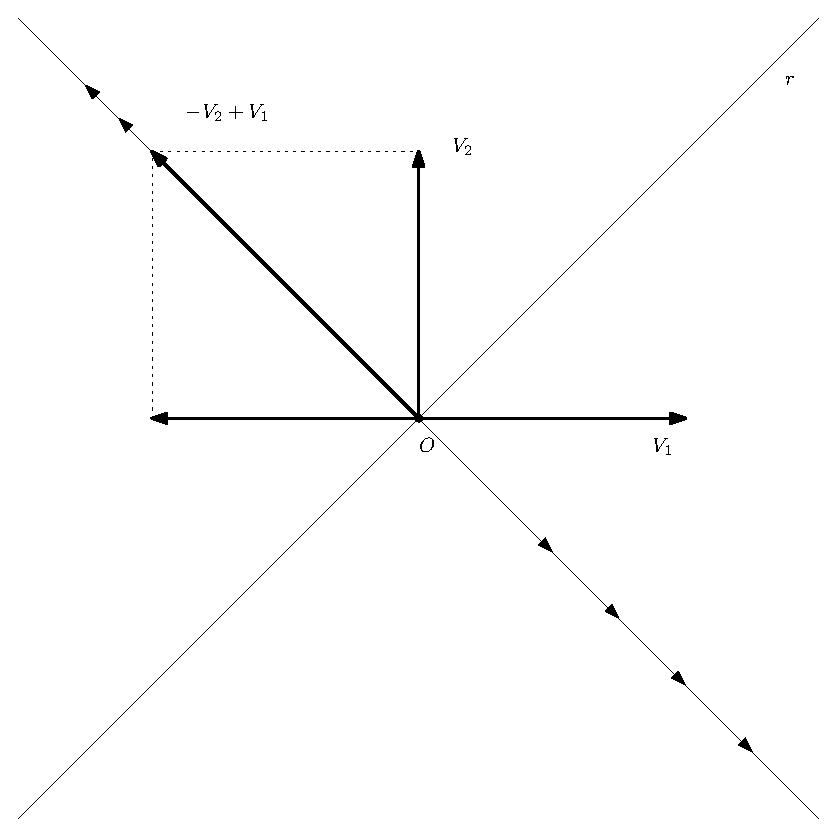
\includegraphics[width=6cm]{img/finiti/imgex4-3-7.eps}
    \end{figure}   
  \item Come ultimo esempio, prendiamo come funzione $f:V_O^2\to V_O^2$ la riflessione rispetto a una retta
    fissata $r$ passante per $O$, ovvero l'endomorfismo che associa a ogni vettore $\vec{OP}$ il suo simmetrico
    rispetto a $r$\footnote{Sappiamo dal primo paragrafo che si tratta di un'applicazione lineare}. Per calcolane
    la matrice associata $M_B(f)$, consideriamo la stessa base $B=\left\{v_1,v_2\right\}$ usata nell'esempio
    precedente.
    \clearpage
    \begin{figure}[th]
      \centering
        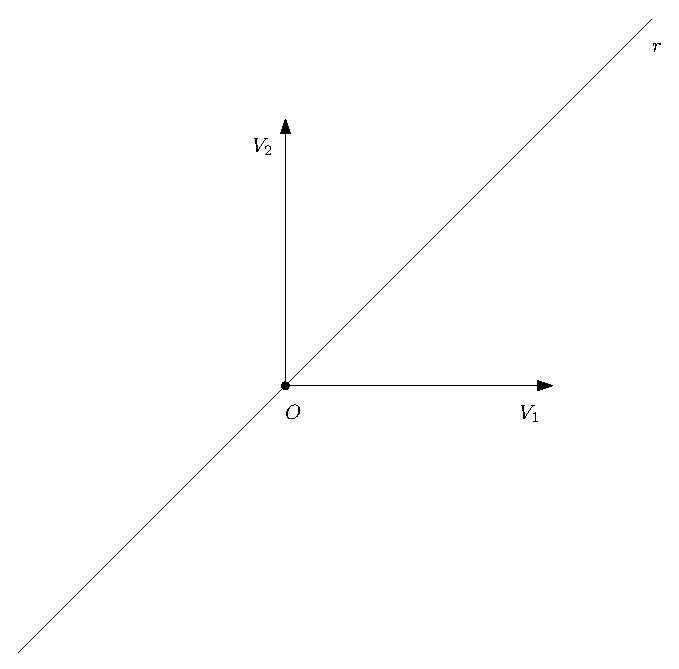
\includegraphics[width=4cm]{img/finiti/imgex4-3-8.eps}
    \end{figure}
    e notiamo che quando riflettiamo $v_1$ rispetto a $r$ otteniamo $v_2$, ovvero $f(v_1)=v_2$, analogamente
    quando riflettiamo $v_2$ rispetto a $r$, otteniamo $v_1$ ovvero $f(v_2)=v_1$.\\
    Quindi, riscrivendo $f(v_1)=v_2$ come $f(v_1)=0v_1+1v_2$ vediamo che le coordinate di $f(v_1)$ rispetto a $B$
    sono $(0,1)$, e analogamente riscrivendo $f(v_2)=v_1$ come $f(v_1)=1v_1+0v_2$ vediamo che le
    coordinate di $f(v_2)$ rispetto a $B$ sono $(1,0)$: disponendo tale coordinate in colonna,
    come previsto dalla definizione della matrice associata, si ottiene
    \begin{equation*}
      M_B(f)=
      \begin{pmatrix}
        0 & 1\\
        1 & 0
      \end{pmatrix}
    \end{equation*}
    Se dato sempre lo stesso endomorfismo, consideriamo invece la base $B^\prime= \{v_1^\prime,
    v^\prime_2$ come nel disegno seguente
    \begin{figure}[th]
      \centering
        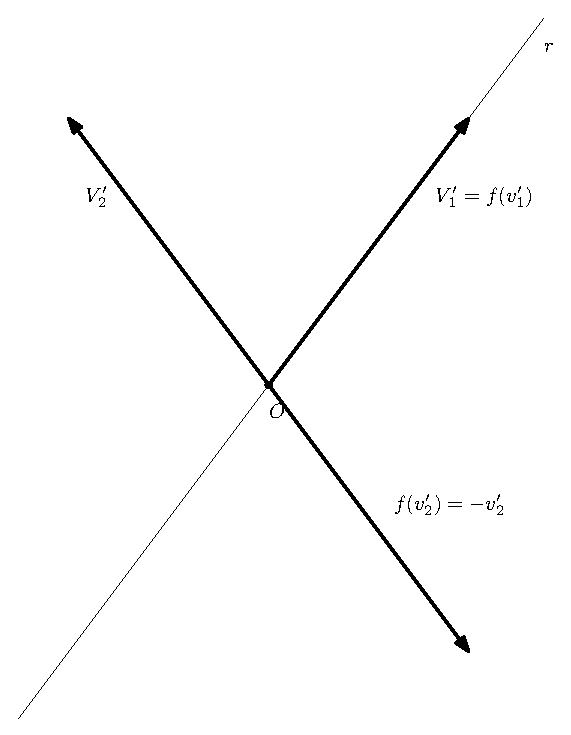
\includegraphics[width=4cm]{img/finiti/imgex4-3-9.eps}
    \end{figure}
    allora si ha che $f(v_1^\prime)=v_1^\prime$ (il vettore $v_1^\prime$ sta sulla retta e quindi
    la riflessione rispetto alla retta lo lascia invariato) e $f(v^\prime_2)=-v^\prime_2$ (il
    vettore $v_2^\prime$ è perpen dicolare alla fetta quindi riflettendolo esso cambia verso),
    cioè $f(v_1^\prime)=1v^\prime_1+0v^\prime_2$ e $f(v_2)=0v_1^\prime+(-1)v_2^\prime$ e quindi
     \begin{equation*}
      M_{B^\prime}(f)=
      \begin{pmatrix}
        1 & 0\\
        0 & -1
      \end{pmatrix}
    \end{equation*}
    Questo esempio illustra il fatto, ovvio che la matrice associata dipenda dalla scelta delle
    basi.
  \end{enumerate}
\end{esempio}

\section{Iniettività e suriettività delle applicazioni lineari}
\label{sec:inie_surie_app_lin}
Il primo problema che affronteremo sulla applicazioni lineari è determinare quando una tale
funzione è iniettiva, suriettiva o biiettiva.

\subsection{Richiami generali}
\label{sec:inie_surie_app_lin_ric_gen}
Ricordiamo che una funzione $f:A\to B$ tra due insiemi $A$ e $B$ si dice \textit{suriettiva} se
ogni elemento del codominio $B$ risulta essere immagine di qualche elemento di $A$ (ovvero, se
per ogni $b\in B$ esiste un $a\in A$ tale che $f(a)=b$).\\
Ad esempio, delle funzioni rappresentate nel seguente disegno, la prima non è
suriettiva\footnote{L'elemento $c\in B$ non è immagine di nessun elemento di $A$},
mentre, la seconda si.
\begin{figure}[th]
  \centering
  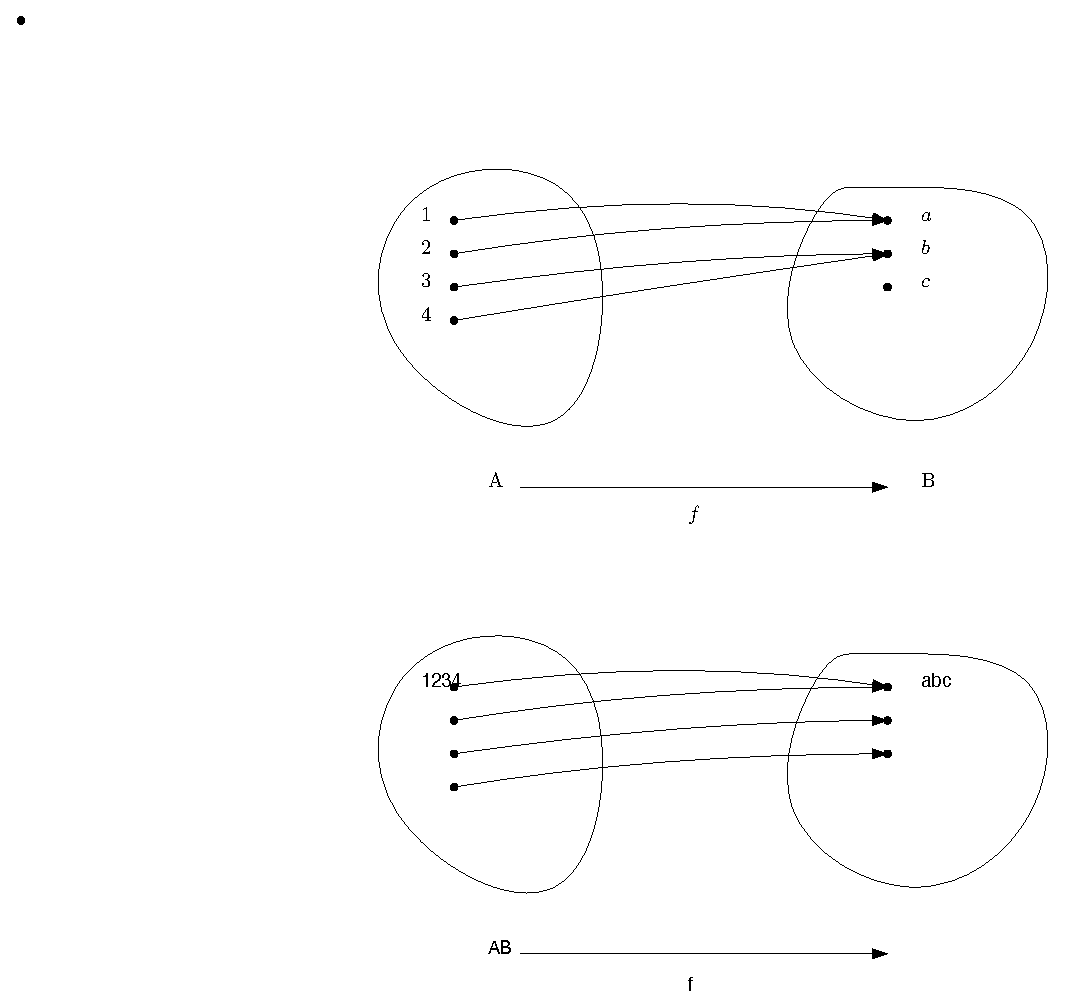
\includegraphics[width=8cm]{img/finiti/imgex4-4-1.eps}
  \caption{differenza tra iniettivo e suriettivo}
\end{figure}
Un modo alternativo di dire che una funzione èsuriettiva è fare riferimento alla cosidetta 
\textit{immagine} $I_m(f)$ di f: per definizione, l'immagine di una funzione $f:A\to B$ è il
sottoinsieme di $B$ costituito da futti gli elementi che sono immagine di qualche elemento di $A$
(in riferimento ai disegni, quegli elementi ``raggiunti da una freccia che provviene da A''),
ovvero
\begin{equation*}
  I_m(f)=\{b\in B | b=f(a) \text{ per qualche } a \in A\}
\end{equation*}
Ad esempio, la funzione sopra nel disegno precedente ha $I_m(f)=\{a,b\}$, mentre la funzione
sotto ha $I_m(f)=\{a,b,c\}$ç una funzione è suriettiva esattamente quando $I_m(f)=B$, ovvero
l'immagine coincide con tutto il codominio\footnote{Dire $I_m(f)=B$ significa in effetti dire
  che ogni elemento di $B$ è immagine di quelche elemento di $A$}.
\begin{figure}[th]
  \centering
  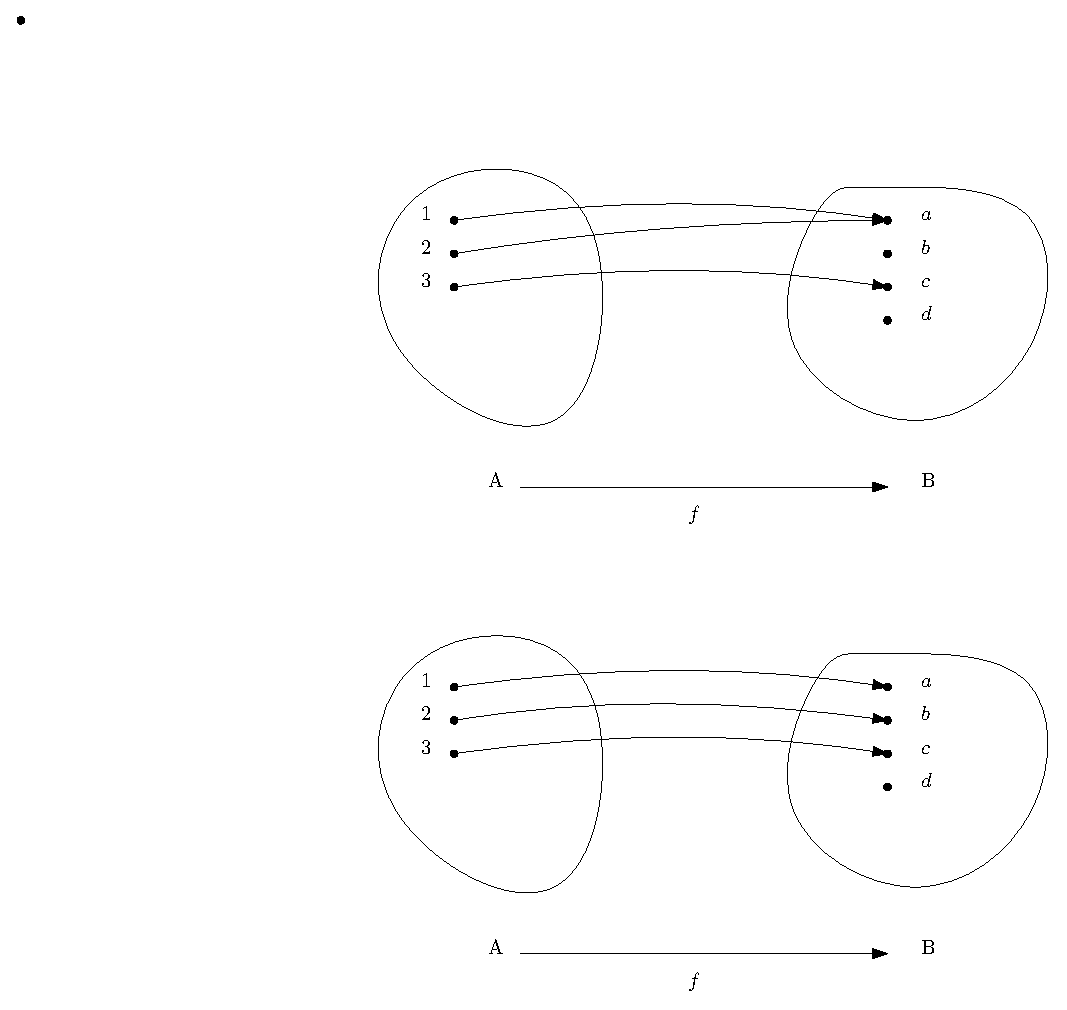
\includegraphics[width=8cm]{img/finiti/imgex4-4-2.eps}
\end{figure}

La nozione di iniettività può essere riformata tramite il concetto di \textit{controimmagine}:
dato un elemento $b$ del codomiono $B$, la sua controimmagine, denotata $f^{-1}(b)$, è l'insieme
di tutti gli elementi di $A$ che hanno $b$ come immagine, ovvero
\begin{equation*}
  f^{-1}(b)=\{a\in A|f(a)=b\}
\end{equation*}
Dal momento che una funzione è iniettiva quando non esistono dhe elementi diversi che hanno la
stessa immagine, dire che una funzione è iniettiva quivale a dire che tutte le controimmagini
che non siano vuote\footnote{se la funzione non è suriettiva, ci saranno elementi $b\in B$ tali
  che non esiste nessun $a\in A$ con $f(a)=b$ e quindi la cui controimmagine $f^{-1}(b)$ non ha
  elementi.} hanno un solo elemento.\\
Ad esempio, per la funzione sofra nel disegno precedente si ha $f^{-1}(a)=\{1,2\},f^{-1}(b)=
\not{0},f^{-1}(c)=\{3\}$: essa non è iniettiva in quanto la controimmagine di a ha due elementi.\\
Per la funzione sotto, invece, si ha $f^{-1}(a)=\{1\}, f^{-1}(b)=\{2\},f^{-1}(c)=\{3\},
f^{-1}(d)=\not{0}$: essa è iniettiva in quanto le controimmagini non vuote hanno tutte un solo
elemento.\\
Infine, una funzione si dice \textit{biiettiva} se è sia inittiva che suriettiva. Ad esempio,
la funzione rappresentata nel sequente disegno è biiettiva.
\begin{figure}[th]
  \centering
  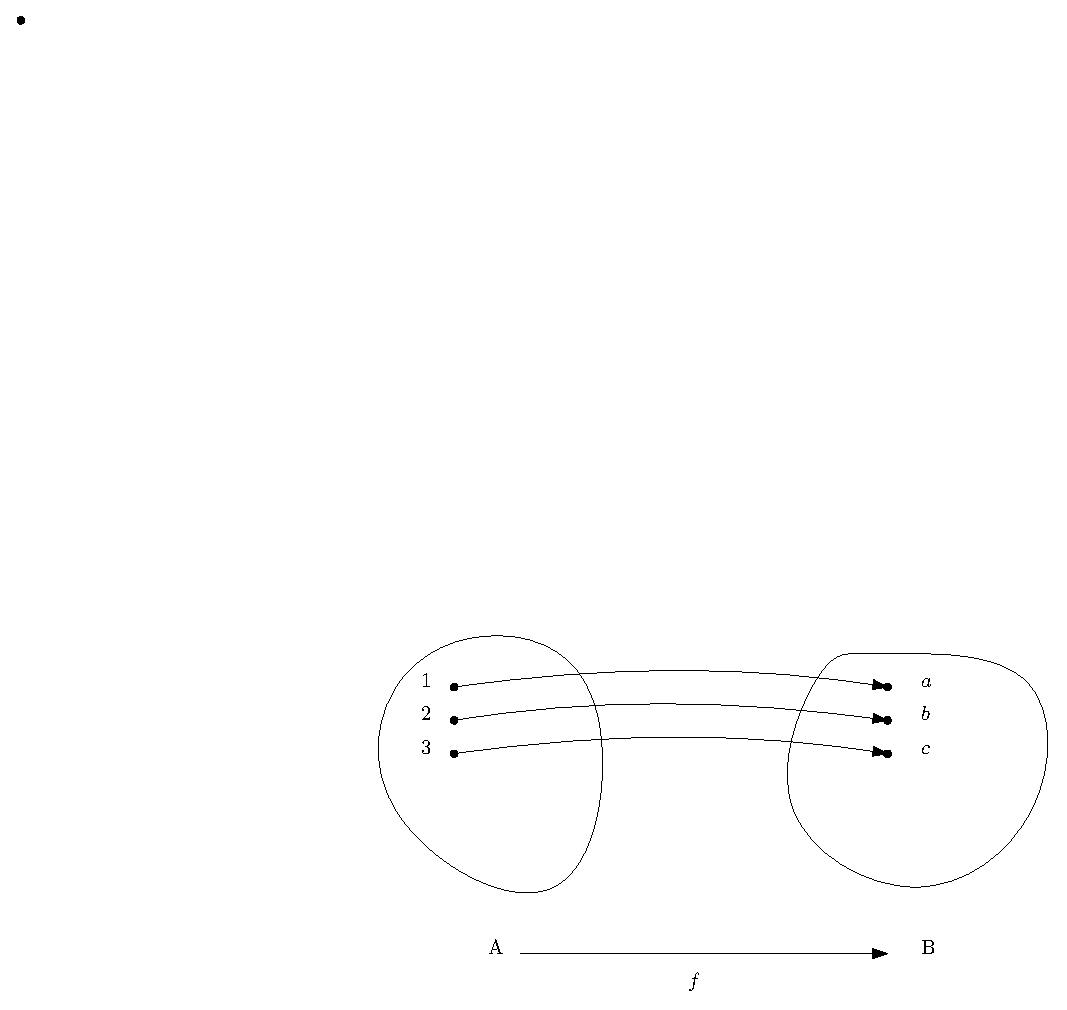
\includegraphics[width=8cm]{img/finiti/imgex4-4-3.eps}
\end{figure}

\subsection{Suriettività delle applicazione lineari}
Abbiamo detto che una funzione $f: A\to B$ è suriettiva se e solo se per ogni elemento di
$b\in B$ esiste un $a\in A$ tale che $f(a)=b$, ovvero equivalentemente se e solo se la sua
immagine $I_m(f)$ coincide con tutto il codominio.\\
Nel caso di un'applicazione lineare $f:V\to W$, vale la seguente importante
\begin{proposizione}
  Sia $f: V\to W$ un'applicazione lineare. Allora $I_m(f)$ è un sottospazio vettoriale di W.
\end{proposizione}
\begin{proof}
  Dobbiamo verificare che $I_m(f)$ è chiuso rispetto alla somma e al prodotto per scalari. Per la
  prima proprietà dobbiamo prendere $w,w^\prime\in I_m(f)$ e vedere se $w+w^\prime\in I_m(f)$. Ora,
  se $w,w^\prime\in I_m(f)$, per definizione di $I_m(f)$ significa che esistono un vettore
  $v\in V$ tale che $w=f(v)$ e un vettore $v^\prime\in V$ tale che $w^\prime=f(v^\prime)$ e un
  vettore $v^\prime\in V$ tale che $w=f(v)$ e un vettore $v^\prime \in V$ tale che
  $w^\prime\in f(v^\prime)$. Ma allora, sfruttando il fatto che $f$ è lineare, si ha
  \begin{equation*}
    w+w^\prime=f(v)+f(v^\prime)=f(v*v^\prime)
  \end{equation*}
  che ci dice che anche $w+w^\prime$ è immagine di un elemento del dominio (cioè $v+v^\prime$) e
  quindi $w+w^\prime\in m(f)$.\\
  Per la chiusura rispetto al prodotto per scalari, dobbiamo verificare che se $w\in I_m(f)$ e
  $c\in\mathds{K}$, allora $cw\in I_m(f)$. Ma, come prima, se $w\in I_m(f)$ allora per
  definizione di $I_m(f)$ esiste un vettore $v\in V$ tale che $w=f(v)$, e quindi, usando sempre
  il fatto che $f$ è linerare,
  \begin{equation*}
    cw=cf(v)=f(cv)
  \end{equation*}
  che ci dice che anche $cw$ è immagine di un elemento del dominio (cioè $cv$) e quindi $cw\in I_m(f)$.
\end{proof}
Il fatto che $I_m(f)$ sia un sottospazio vettoriale ci dice che per determinarla possiamo trovarne un sistema di
generatori o una base. Questo si fa facilmente grazie alla seguente
\begin{proposizione}
  Sia $f:V\to W$ un'applicazione lineare e siamo $v_1,\dots,v_n$ generatori $V$.
  Allora le immagini $f(v_1),\dots,f(v_n)$ generano $I_m(f)$ (in simboli, $I_m(f)=[f(v_1),\dots,f(v_n)]$)
\end{proposizione}
\begin{proof}
  Per definizione di generatori, dobbiamo verificare che ogni vettori $w\in I_m(f)$ si può scrivere come
  combinazione lineare dei vettori $f(v_1),\dots,f(v_n)$. Ora, sappiamo che un vettore $w\in I_m(f)$ è tale che
  $w\in f(v)$ per qualche $v\in V$. Ma essendo per ipotesi $v_1,\dots,v_n$ generatori di $V$, il vettore
  $v$ potrà essere scrittocome loro combinazione lineare $v=x_1v_1+\dots+x_nv_n$. Quindi, sfruttando la
  linearità di $f$ si ha
  \begin{equation*}
    w=f(v)=f(x_1v_1+\dots+x_nv_n)=x_1f(v_1)+\dots+x_nf(v_n)
  \end{equation*}
  che dimostra prprio che $w$ si scrive come combinazione lineare di $f(v_1),\dots,f(v_n)$, come volevamo.
\end{proof}
A questo punto, per determinare se un'applicazione lineare $f:V\to W$ è suriettiva, basta scegliere dei
generatori $v_1,\dots,v_n$ di $V$, prendere le loro immagini $f(v_1),\dots,f(v_n)$ che, come abbiamo appena
visto, formano un insieme di generatori di $I_m(f)$, e poi estrarre da quest'ultimo insieme una base eliminando
gli eventuali vettori che sono dipendenti dai rimanenti: contando i vettori della base ottenuta, sapremo la
dimensione di $I_m(f)$ e quindi $f$ sarà suriettiva se e solo se\footnote{Questa affermazione è giustificato
  dal fatto, che non abbiamo dimostrato, che se $S$ è un sottospazio vettoriale di una spazio vettoriale $V$,
  allora $dim (S)\leq dim (V)$ e le dimensioni coincidono se e solo se $S=V$.} $dim(I_m(f))=dim(W)$.\\
Vediamo come tale criterio di suriettività si rivela particolarmente utile e di semplice applicazione nel caso
dell'applicazioni lineare $L_A:\mathds{K}^n\to \mathds{K}^m$ determinata da una matrice $A$, ovvero della forma
data dalla (4.9)\footnote{Come sappiamo, ogni applicazione lineare puo`essere identificata con una tale
  funzione grazie alla matrice associata}.\\
Ora, se come generatori del dominio $V=\mathds{K}^n$ scegliamo i vettori della base canonica
$v_1=(1.0.\dots,0),v_2=(0,1,\dots,0),v_n=(0,0,\dots,1)$, dalla (4.9) si ha
\begin{equation*}
  f(v_1)=L_A
  \begin{pmatrix}
    1 \\
    0 \\
    \vdots\\
    0
  \end{pmatrix}=
  \begin{pmatrix}
    a_{11}\\
    a_{12}\\
    \vdots\\
    a_{m1}
  \end{pmatrix},
  f(v_2)= L_A
   \begin{pmatrix}
    0 \\
    1 \\
    \vdots\\
    0
   \end{pmatrix}=
   \begin{pmatrix}
    a_{12}\\
    a_{22}\\
    \vdots\\
    a_{m2}
   \end{pmatrix}, \dots, f(v_n)=
   L_A
   \begin{pmatrix}
    0\\
    0\\
    \vdots\\
    1
   \end{pmatrix}=
   \begin{pmatrix}
    a_{1n}\\
    a_{2n}\\
    \vdots\\
    a_{mn}    
   \end{pmatrix}
\end{equation*}
cioè $f(v_1),f(v_2),\dots,f(v_n)$ sono le colonne $C_1,C_2,\dots,C_n$ della matrice $A$ che determina
l'applicazione. Quindi, in base alla Proposizione \textbf{2}, si ha $I_m(f)=\{C_1,c_2,\dots,C_n\}$ e la funzione
è suriettiva se e solo se $dim\{C_1,C_2,\dots,C_n\}=dim(\mathds{K}^m)=m$. Ma poiché la dimensione del sottospazio
generato dalle colonne di una metrice è per definizione il suo rango, concludiamo che \textit{un'applicazione
  del tipo (4.9) è suriettiva se e solo se il rango di $A$ è uguale a $m$}.

\subsection{Iniettività di applicazioni lineari}
Mentre nel caso della suriettività abbiamo visto che per verificare se una funzione $f$ è suriettiva basta
controllare un solo sottoinsieme del codomonio (l'immagine $I_m(f)$), in generale per verificare se $f$ è
iniettiva dobbiamo a priori controllare tutte le controimmagini degli elementi del codominio e verificare che
queste, quando non sono vuote, hanno un solo elemento.\\
Ora, per una generica funzione $f:A\to B$ le controimmagini degli elementi di $B$ sono sottoinsiemi del tutto
indipendenti tra loro: come nel seguente disegno
\begin{figure}[th]
  \centering
  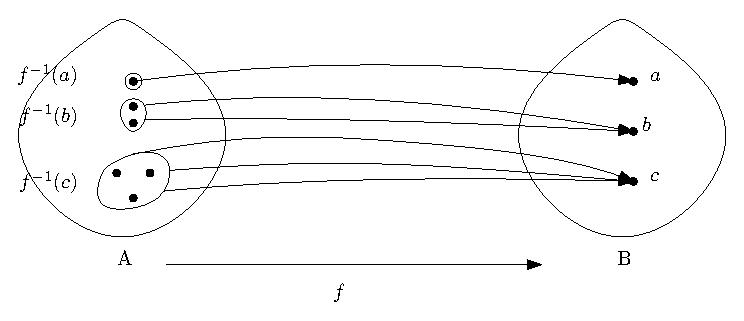
\includegraphics[width=8cm]{img/finiti/imgex4-4-4.eps}
\end{figure}

può accadere che un elemento abbia controimmagine costituine costituita da un solo elemento ma altri abbiamo
controimmagine costituita da più elementi. Vedremo ora invece che le applicazioni lineari hanno il particolare
comportamento per cui le controimmagini degli elementi di $B$, se non sono vuote, o sono \textit{tutte}
costituite da un solo elemento (nel quel caso la funzione non è iniettiva): quindi basta controllare una sola
controimmagine non vuota per capire come sono fatte tutte le altre. Più precisamente abbiamo la seguente
\begin{proposizione}
  Sia $f: V\to W$ un'applicazione lineare. Allora valgono i seguenti fatti:
  \begin{description}
  \item[(i)] la controimmagine $f^{-1}(\bar{0})=\{v\in V | f(v)=\bar{0}\}$ del vettore nullo di $W$ è un
    sottomatrice vettoriale di $V$ (detto \textit{nucleo di} $f$ denotato $N(f)$)
  \item[(ii)] per ogni $w_0\in W$, la controimmagine $f^{-1}(w_0)$ di $w_0$,  non è vuota, è un sottospazio
    affine di $V$, e più precisamente
    \begin{equation*}
      f^{-1}(w_0)=v_0+N(f)=\{v_0+n|n\in N(f)\}
    \end{equation*}
    dove $v_0$ è un qualunque elemento fissato d $f^{-1}(w_0)$.
  \end{description}
\end{proposizione}
\begin{proof}
  Per dimostrare $(i)$, iniziamo con l'osservare che il nucleo di $f$ non è mai vuoto, in quanto il vettore
  nullo di $V$ (che, con un abuso di notazione, denotiamo ancora $\bar{0}$) è sicuramente tale che
  $f(\bar{0})=\bar{0}$: infatti, possiamo il vettore nullo $\bar{0}$ di $V$ come $0v$ (dove $v$ è un qualunque
  vettore di $V$) e quindi, sfruttando la linearità di $f$, si ha $f(\bar{0})=f(0v)=0f(v)=\bar{0}$.\\
  Siano $v,v^\prime$ due vettori di $N(f)$, cioè $f(v)=\bar{0}$. Allora, essendo $f$ lineare,
  \begin{eqnarray*}
    f(v+v^\prime)=f(v)+f(v^\prime)=\bar{0}+\bar{0}=\bar{0}
  \end{eqnarray*}
  e quindi anche $v+v^\prime\in N(f)$: questo ci dice che $N(f)$ è chiuso rispetto alla somma.
  Dati invece un vettore $v$ del nucleo\footnote{quindi $f(v)=\bar{0}$} e uno scalare $c\in
  \mathds{K}$, allora, sempre per la linearità di $f$,
  \begin{eqnarray*}
    f(cv)=cf(v)=c\bar{0}=\bar{0}
  \end{eqnarray*}
  ovvero $cv\in N(f)$: questo ci dice che $N(f)$ chiuso rispetto al prodotto per scalari -- La
  \textit{(i)} è dimostrata.\\
  Per dimostrare la \textit{(ii)}, ovvero l'ugualianza $v=N(f)=f^{-1}(w_0)$, dobbiamo dimostrare
  che ogni elemento di $v_0+N(f)$ sta nella controimmagine $f^{-1}(w_0)$ appartiene a $v_0+N(f)$
  (ovvero l'inclusione opposta $f^{-1}(w_0)$). Per dimostrare la prima inclusione, consideriamo il
  generico elemento di $v_0=N(f)$, cioè, per definizione di sottospazio affine, un vettore $v$ del
  tipo $v=v_0+n$, con $n\in N(f)$. Allora
  \begin{equation*}
    f(v)=f(v_0+n)=f(v_0)+f(n)=f(v_0)=\bar{0}=f(v_0)=w_0
  \end{equation*}
  (nella seconda uguaglianza abbiamo usato il fatto che $f$ è lineare, nella terza il fatto che $n$ appartiene
  al nucleo di $f$ e quindi $f(n)=\bar{0}$). Abbiamo dimostrato che $f(v)=w_0$, cioè $v$ appartiene alla
  controimmagine $f^{-1}(w_0)$ di $w_0$, come volevamo.\\
  Per dimostrare la seconda inclusione, consideriamo un qualunque elemento $v$ della controimmagine di $w_0$,
  cioè $f(v)=w_0$. Essendo $w_0=f(v_0)$, si ha quindi $f(v)=f(v_0)$, da cui, portando a primo membro,
  $f(v)-f(v_0)=\bar{0}$. Essendo $f$ lineare, quest'ultima uguaglianza può essere riscritta $f(v-v_0)=\bar{0}$,
  il che ci dice che il vettore $v-v_0$ appartiene al nucleo $N(f)$ di $f$. Ma allora, osservando che chiaramente
  $v=v_0+(v-v_0)$, vediamo che $v$ si decompone proprio come somma di $v_0$ e di un elemento del nucleo $N(f)$,
  $v\in v_0+N(f)$, come volevamo.
\end{proof}
La proposizione appena dimostrata afferma in pratica che tutte le controimmagini non vuote
di un'applicazione lineari $f$ sono ``copie'' o traslati del nucleo $N(f)$: per illustrare ciò,
consideriamo ad esempio lo spazio $V_0^2$ dei vettori nel piano applicati in = e l'applicazione
lineare $f:V^2_O \to V^2_O$ data dalla proiezione ortogonale su una retta $r$ fissata.\\
Come si vede, un vettore viene proiettato sul vettore nullo $\vec{OO}$ (cioè appartiene al
nucleo $N(f)$ della funzione) se e solo se appartiene alla retta passante per $O$ e ortogonale
a $r$, come i vettori $\vec{OP}. \vec{OQ}$ del disegno sequente
\begin{figure}[th]
  \centering
  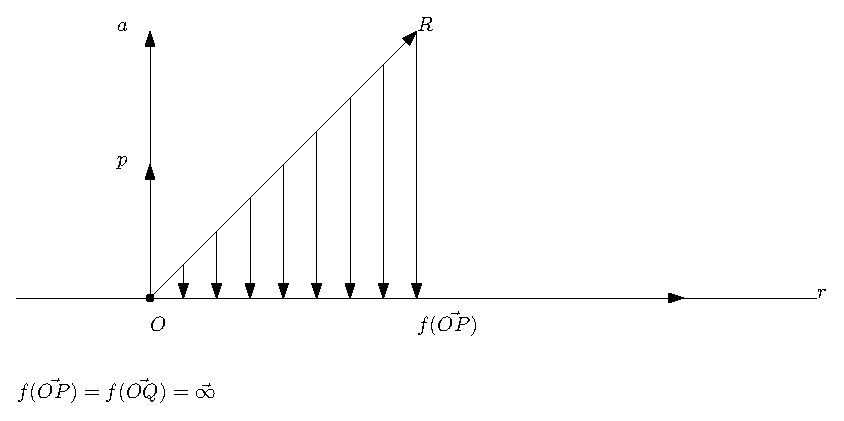
\includegraphics[width=8cm]{img/finiti/imgex4-4-5.eps}
\end{figure}

Ma, come sappiamo, i vettori che stanno su una retta per $O$ formano un sottospazio vettoriale:
questo conferma che il nucleo N(f) è un sottospazio vettoriale.
Per verificare ora che le contro immagini non vuote sono copie traslati del nucleo, consideriamo
come nel disegno seguente
\begin{figure}[th]
  \centering
  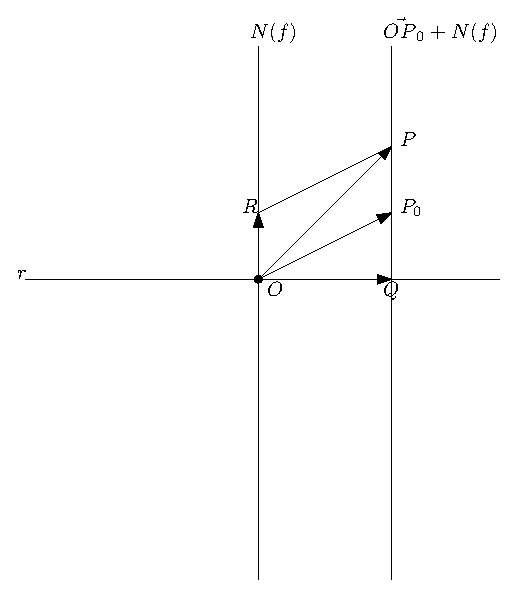
\includegraphics[width=5cm]{img/finiti/imgex4-4-6.eps}
\end{figure}

Un qualunque vettore $\vec{OP}$ che stia nell'immagine di $f$, diciamo $\vec{OQ}=f(\vec{OP}_0)$:
la sua controimmagine, oltre che da $\vec{OP}_0$, è data da tutti i vettori $\vec{OP}$ che
vengono proiettati su $\vec{OQ}$, cioè, come si vede nel disegno, tutti i vettori che hanno
secondo estremo sulla retta ortogonale a $r$ e passante per $Q$.
\clearpage
